\section{Durchführung}
\label{sec:Durchführung}


Für den Versuch wird ein Aufbau gemäß Abbildung \ref{fig:aufbau} verwendet.

\begin{figure}
    \centering
    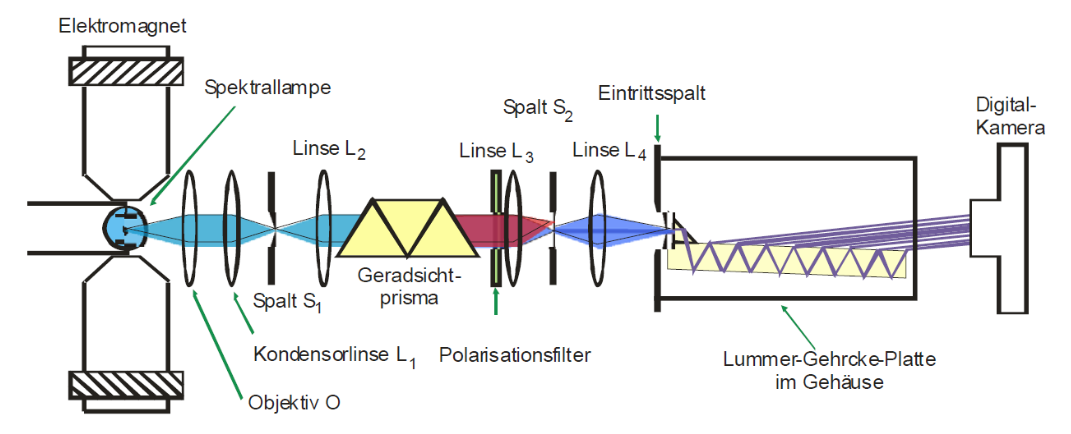
\includegraphics[width=\textwidth]{Bilder/Aufbau.PNG}
    \caption{Schematischer Versuchsaufbau.}
    \label{fig:aufbau}
\end{figure}

Da es im Rahmen des Versuchs, keine Möglichkeit gibt, das Magnetfeld während des Versuchs zu messen, wird der Elektromagent geeicht. Dazu wird die Feldstärke des B-Feldes, mit Hilfe einer in das Feld eingeführten Hall-Sonde, in Abhängigkeit des Stroms gemessen. So kann auch ohne Hall-Sonde, über den Strom auf die Feldstärke des Magneten rückgeschlossen werden.



Für eine möglichst genaue Messung muss der Aufbau zunächst justiert werden. Die Justage wird an der Cd-Lampe begonnen und der Reihenfolge der Bauteile nach durchgeführt. 
Als erstes wird das Licht der Cd-Lampe über ein Objektiv und einer Linse scharf auf den ersten Spalt $S_1$ abgebildet.
Daraufhin wird das Licht in der Linse $L_2$ so gebrochen, dass ein möglichst paralleles Lichtbündel entsteht, welches dann mit wenig Verlust in das Geradsichtprisma fällt. Dazu sollte der Durchmesser des Lichtsbündels die größe des Prismas nicht übersteigen. 
Über die Linse $L_3$ werden die Lichtstrahlen, die das Prisma verlassen, scharf auf den Spalt $S_2$ abgebildet. Über diesen Spalt kann dann eine Selektion der einzelnen Spektrallinien vorgenommen werden. Über die Justage der Linse $L_4$ wird ein scharfes Bild auf die Lummer-Gehrcke-Platte geworfen. Auch hier wird darauf geachtet, dass das Bild der Größe des Eintritts-Prismas entspricht. 
Nun wird ein Polarisator in dem Strahlengang platziert, welcher, je nach Stellung, den jeweiligen Übergang ($\Delta m = \pm1,0$) ausblendet.
Am Ende des Aufbaus ist eine, auf die Lummer-Gehrcke-Platte gerichtete, Kamera angebracht, mit der die aufgespalteten Linien fotografiert werden können. Damit ist der Aufbau und die Justage abgeschlossen und der eigentliche Messvorgang kann beginnen. 


Zuerst wird die rote Linie betrachtet. Dazu wird der Spalt $S_2$ auf die rote Linie geschoben. Durch eine Verschiebung des Spalten kann es vorkommen, dass die folgenden Bauteile erneut nachjustiert werden müssen. Dies gilt auch für die späteren Messungen der blauen Linie.
Daraufhin wird bei ausgeschaltetem B-Feld das Spektrum der roten Linie fotografiert. Das B-Feld wird über einen Strom von $I=\SI{5.03}{\ampere}$ auf $B=\SI{0.441}{\tesla}$ eingestellt und es werden Fotos in Abhängigkeit der Stellung des Polarisationsfliter erstellt. Bei einer Polarisator-Stellung von $\SI{0}{\degree}$ wird das $\sigma$-polarisierte Licht ausgeblendet und bei einer Polarisator-Stellung von $\SI{90}{\degree}$ wird das $\pi$-polarisierte Licht ausgeblendet.
Dieser Vorgang wird analog für die blaue Linie durchlaufen. Für die $\sigma$-Linie wird das B-Feld auf $B=\SI{0.314}{\tesla}$ und für die $\pi$-Linie auf $B=\SI{0.441}{\tesla}$ gestellt. Diese genauen Werte folgen aus der in Abschnitt \ref{sec:Auswertung} durchgeführten Ausgleichsrechnung. Beim der Durchführung können nur die jeweils dazu passenden Stomstärken eingestellt werden. Auf diese Weise werden also ingesamt sechs Bilder aufgenommen, welche jeweils vom B-Feld und der Stellung des Polarisators abhängen.

 %Was wurde gemessen bzw. welche Größen wurden variiert?